\documentclass[12pt,a4paper,twoside,openright]{report}
\usepackage{Thesis_template}

%\usepackage{fancyhdr}
%\pagestyle{fancy}
%\fancyhf{}
%\fancyhead[R]{\thepage}

\newcommand\PaperTitleOne{Saddlepoint-adjusted inversion of characteristic functions}
\newcommand\PaperTitleTwo{An information criterion for automatic gradient tree boosting}
\newcommand\PaperTitleThree{agtboost: Adaptive and Automatic Gradient Tree Boosting Computations}
%\newcommand\PaperTitleFour{The Fourth Paper}

%\usepackage{amsthm}
%\theoremstyle{definition}
%\newtheorem{exmp}{Example}[section]

%\usepackage{amsmath}
\newtheorem{Example}{Example}[section]
\usepackage{romannum}

%algorithm
\usepackage{rotfloat}
\providecommand{\tabularnewline}{\\}
\floatstyle{ruled}
\newfloat{algorithm}{tbp}{loa}
\providecommand{\algorithmname}{Algorithm}
\floatname{algorithm}{\protect\algorithmname}

\newcommand{\features}{\ensuremath{\mathbf{x}}}

\begin{document}

%%%%%%%%%%%%%%%%%%%%%%% TITLE PAGE %%%%%%%%%%%%%%%%%%%%%%%%%%%%%%%%%%%%%%%
\title{Information in Local Curvature:\linebreak{}
	Three Papers on Adaptive Methods\linebreak{}
	in Computational Statistics}
\author{Berent Ånund Strømnes Lunde}
\year{2020}
\faculty{Faculty of Science and Technology}
\department{Department of Mathematics and Physics}

\insertTitlePage

%%%%%%%%%%%%%%%%%%%%%%%%%%%%%%% COLOPHON %%%%%%%%%%%%%%%%%%%%%%%%%%%%%%%%%

\ISBN{}
\ISSN{}
\thesisnum{}

\insertColophon

%%%%%%%%%%%%%%%%%%%%%%%%%%%%%%%%%%%%%%%%%%%%%%%%%%%%%%%%%%%%%%%%%%%%%%%%%%
\fontdimen2\font=4pt % Inter word space
%%%%%%%%%%%%%%%%%%%%%%%%%%%%% PREFACE %%%%%%%%%%%%%%%%%%%%%%%%%%%%%%%%%%%%

\includePage{Preface}{Preface}


%%%%%%%%%%%%%%%%%%%%%%%%%%%% ACKNOWLEDGEMENTS %%%%%%%%%%%%%%%%%%%%%%%%%%%%%%%%%%%%

\includePage{Acknowledgements}{Acknowledgements}


%%%%%%%%%%%%%%%%%%%%%%%%%%%% ABSTRACT %%%%%%%%%%%%%%%%%%%%%%%%%%%%%%%%%%%%

\includePage{Abstract}{Abstract}

%%%%%%%%%%%%%%%%%%%%%%%%%%%% LIST OF PAPERS %%%%%%%%%%%%%%%%%%%%%%%%%%%%%%

%\includePage{Paper_list}{List of papers}

%%%%%%%%%%%%%%%%%%%%%%% TABLE OF CONTENTS %%%%%%%%%%%%%%%%%%%%%%%%%%%%%%%%

\insertTOC

%%%%%%%%%%%%%%%%%%%%%%%%%%%% PAGE STYLES %%%%%%%%%%%%%%%%%%%%%%%%%%%%%%%%%

\setPageStyles

%%%%%%%%%%%%%%%%%%%%%%%%%% INTRODUCTION %%%%%%%%%%%%%%%%%%%%%%%%%%%%%%%%%%

\includeChapter{Introduction}
\includeChapter{ML_and_SL}
\includeChapter{Quadratics}
\includeChapter{Computation}
\includeChapter{Summary}

%%%%%%%%%%%%%%%%%%%%%%%%%%% REFERENCES %%%%%%%%%%%%%%%%%%%%%%%%%%%%%%%%%%%

\displayReferences{Thesis_bib}

%%%%%%%%%%%%%%%%%% TABLE OF CONTENTS, APPENDIX %%%%%%%%%%%%%%%%%%%%%%%%%%%

\insertTOCA

%%%%%%%%%%%%%%%%%%%%%%%%%%%%%%% PAPER I %%%%%%%%%%%%%%%%%%%%%%%%%%%%%%%%%%

\insertPaper{I}{\PaperTitleOne}
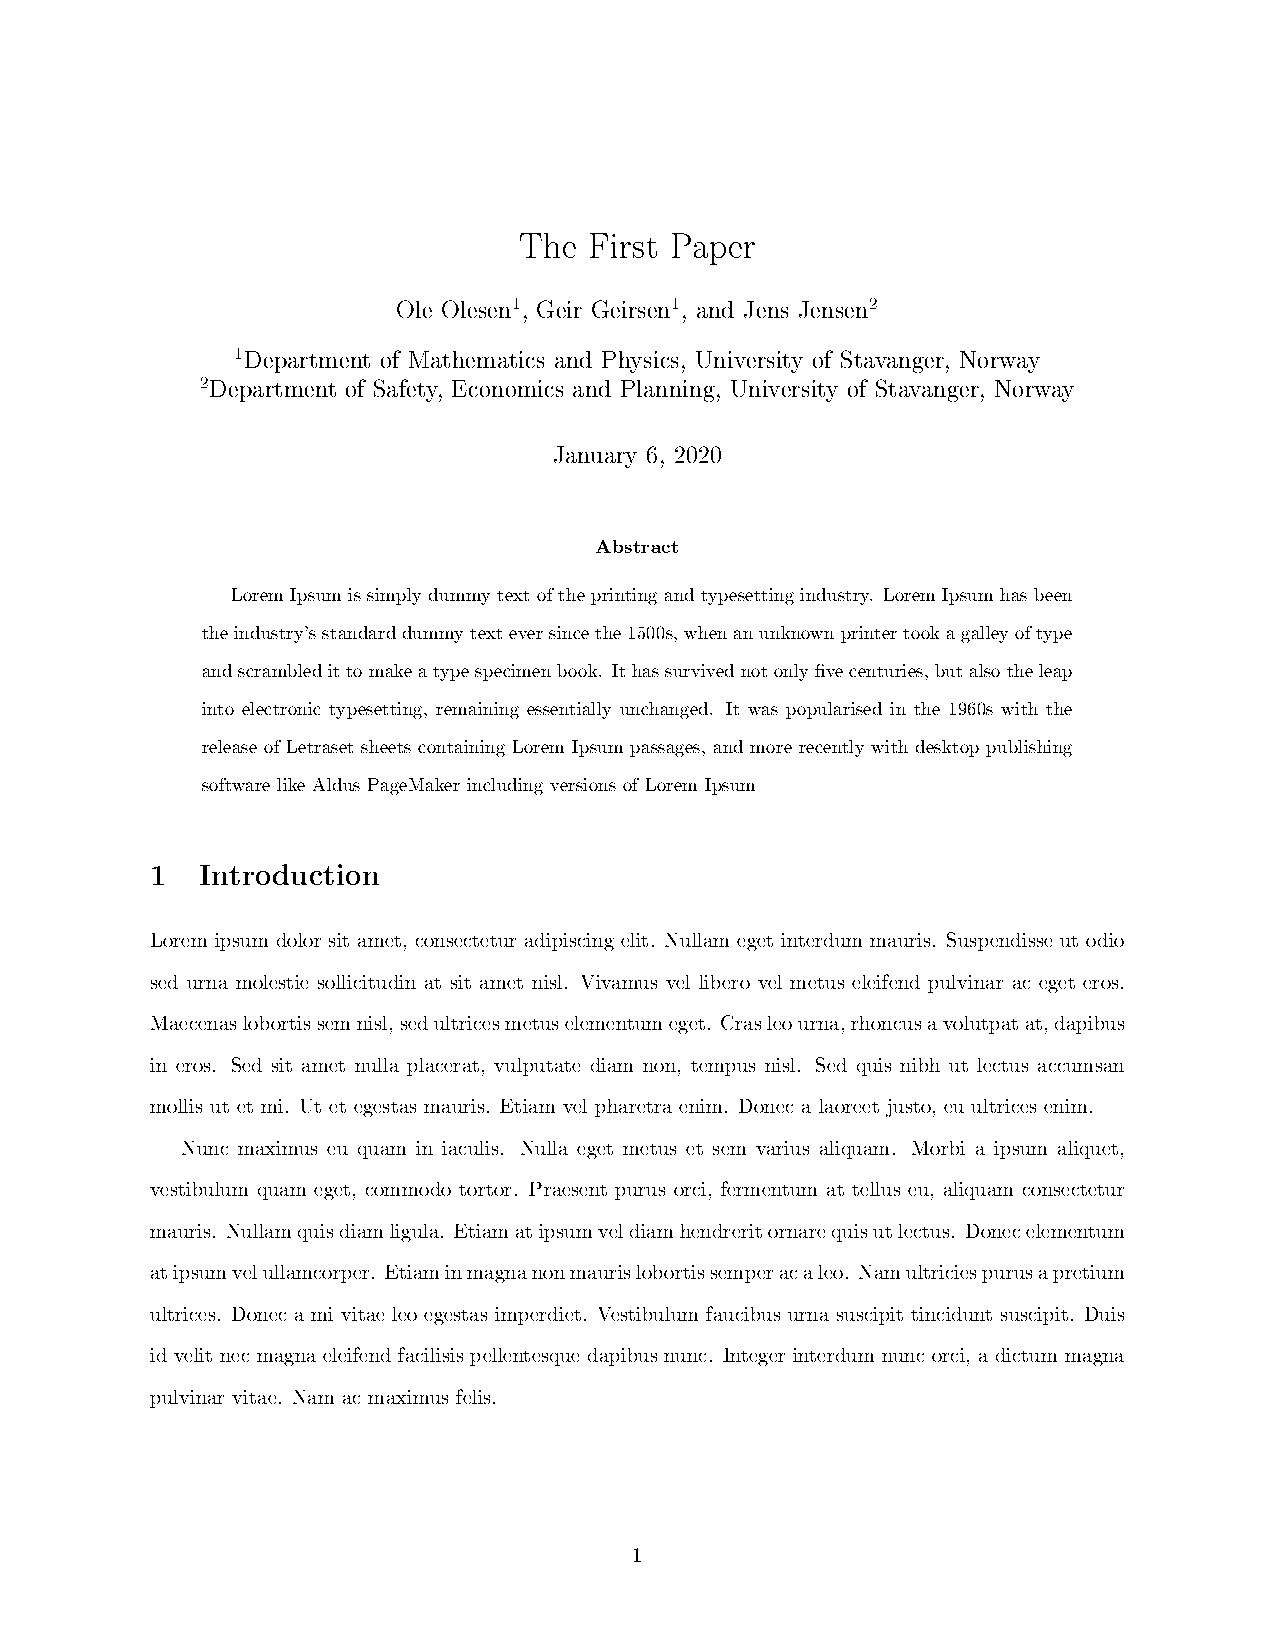
\includepdf[pages=-,scale=0.74,offset=0mm 0mm,pagecommand={\thispagestyle{plain}}]{papers/Paper1.pdf}

%%%%%%%%%%%%%%%%%%%%%%%%%%%%%%% PAPER II %%%%%%%%%%%%%%%%%%%%%%%%%%%%%%%%%

\insertPaper{II}{\PaperTitleTwo}
%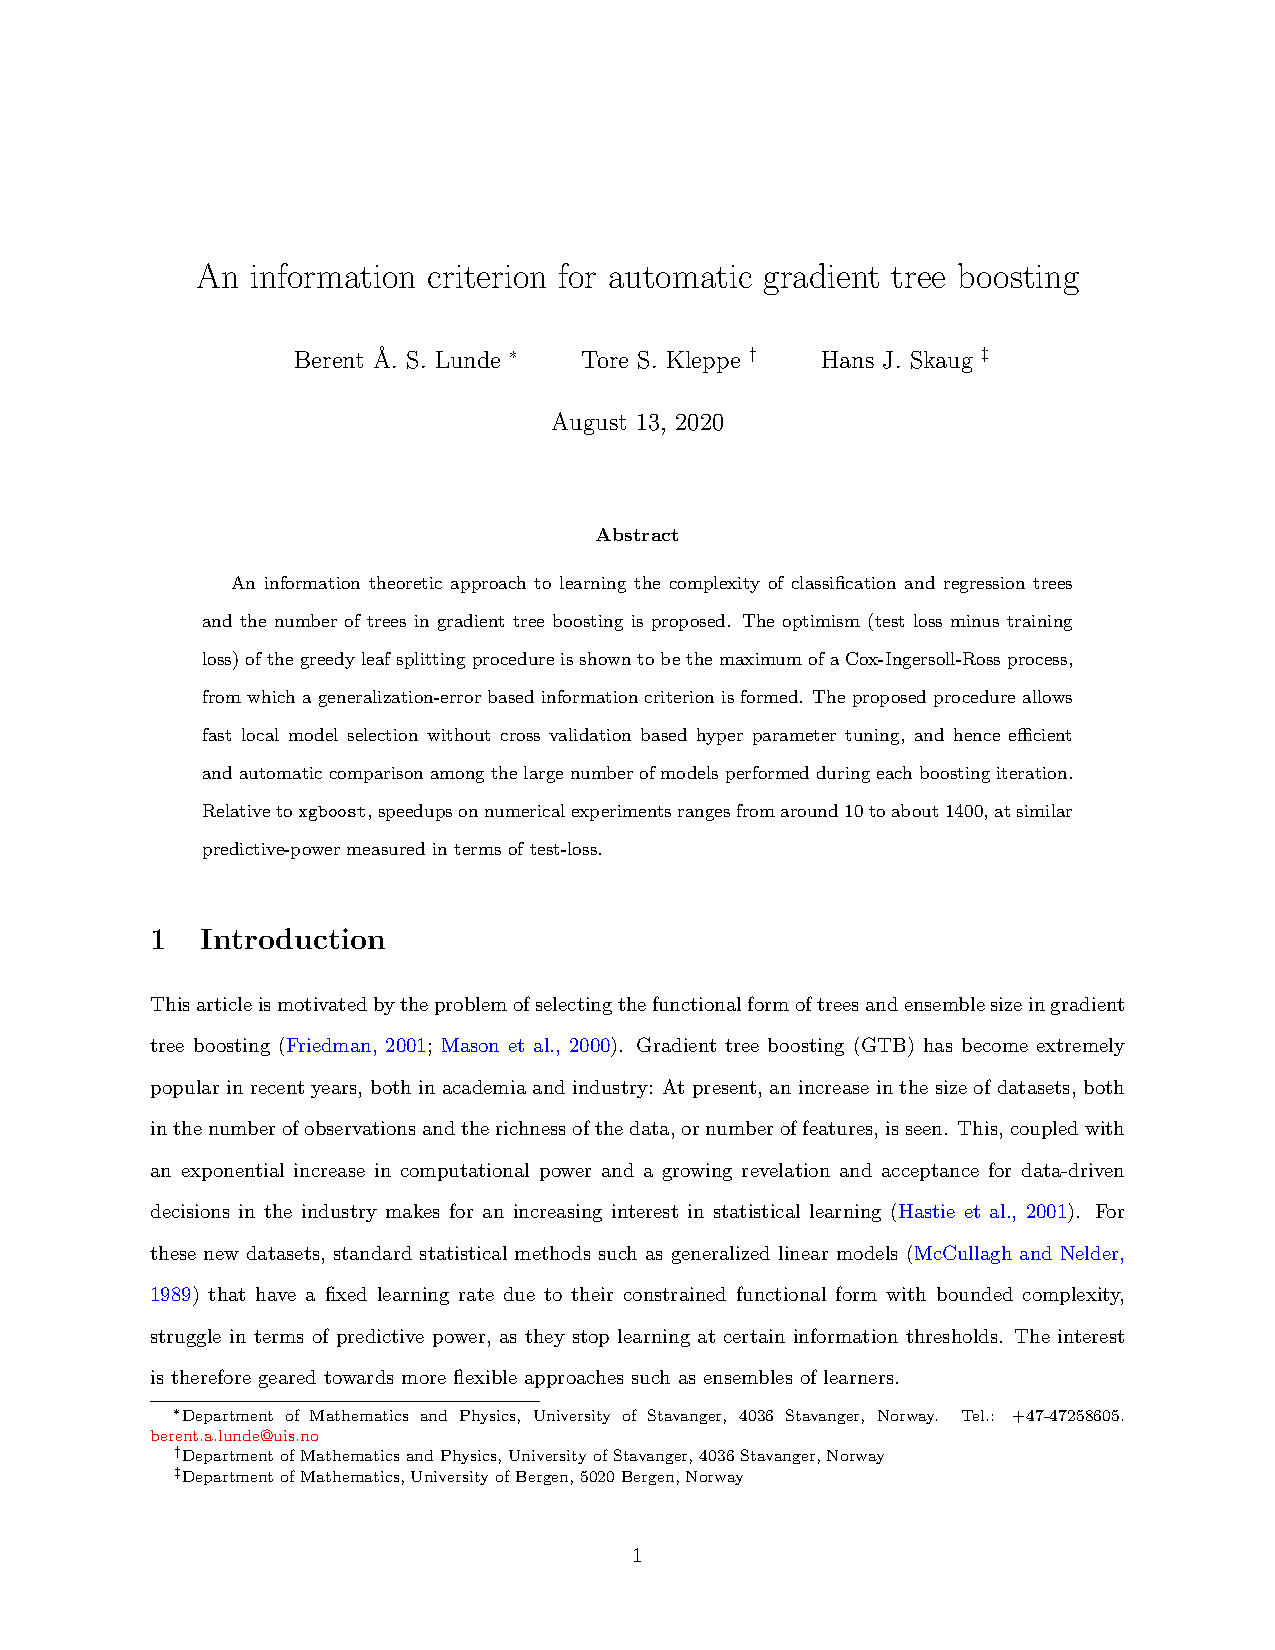
\includepdf[pages=-,scale=0.74,offset=0mm -10mm,pagecommand={\thispagestyle{plain}}]{papers/Paper2.pdf}
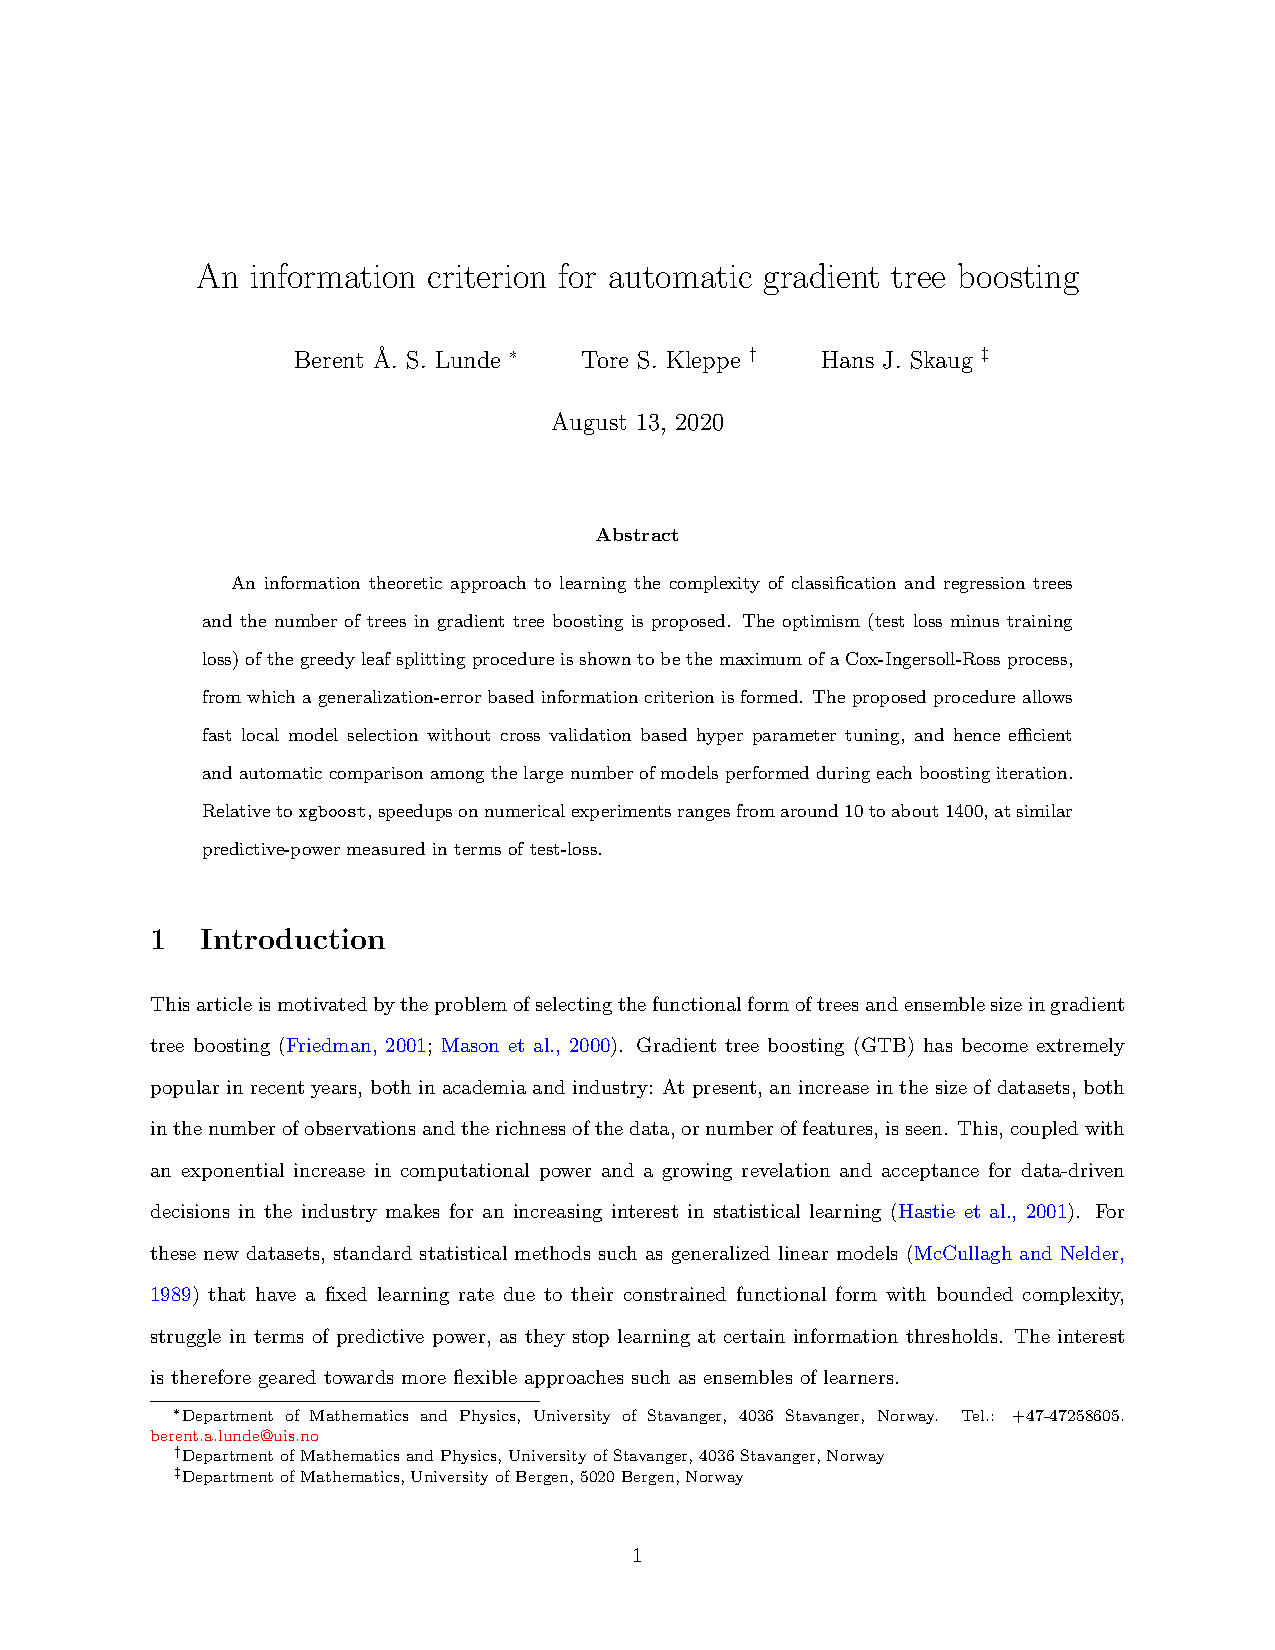
\includepdf[pages=-,scale=0.74,offset=0mm 0mm,pagecommand={\thispagestyle{plain}}]{papers/Paper2.pdf}

%%%%%%%%%%%%%%%%%%%%%%%%%%%%%%% PAPER III %%%%%%%%%%%%%%%%%%%%%%%%%%%%%%%%

\insertPaper{III}{\PaperTitleThree}
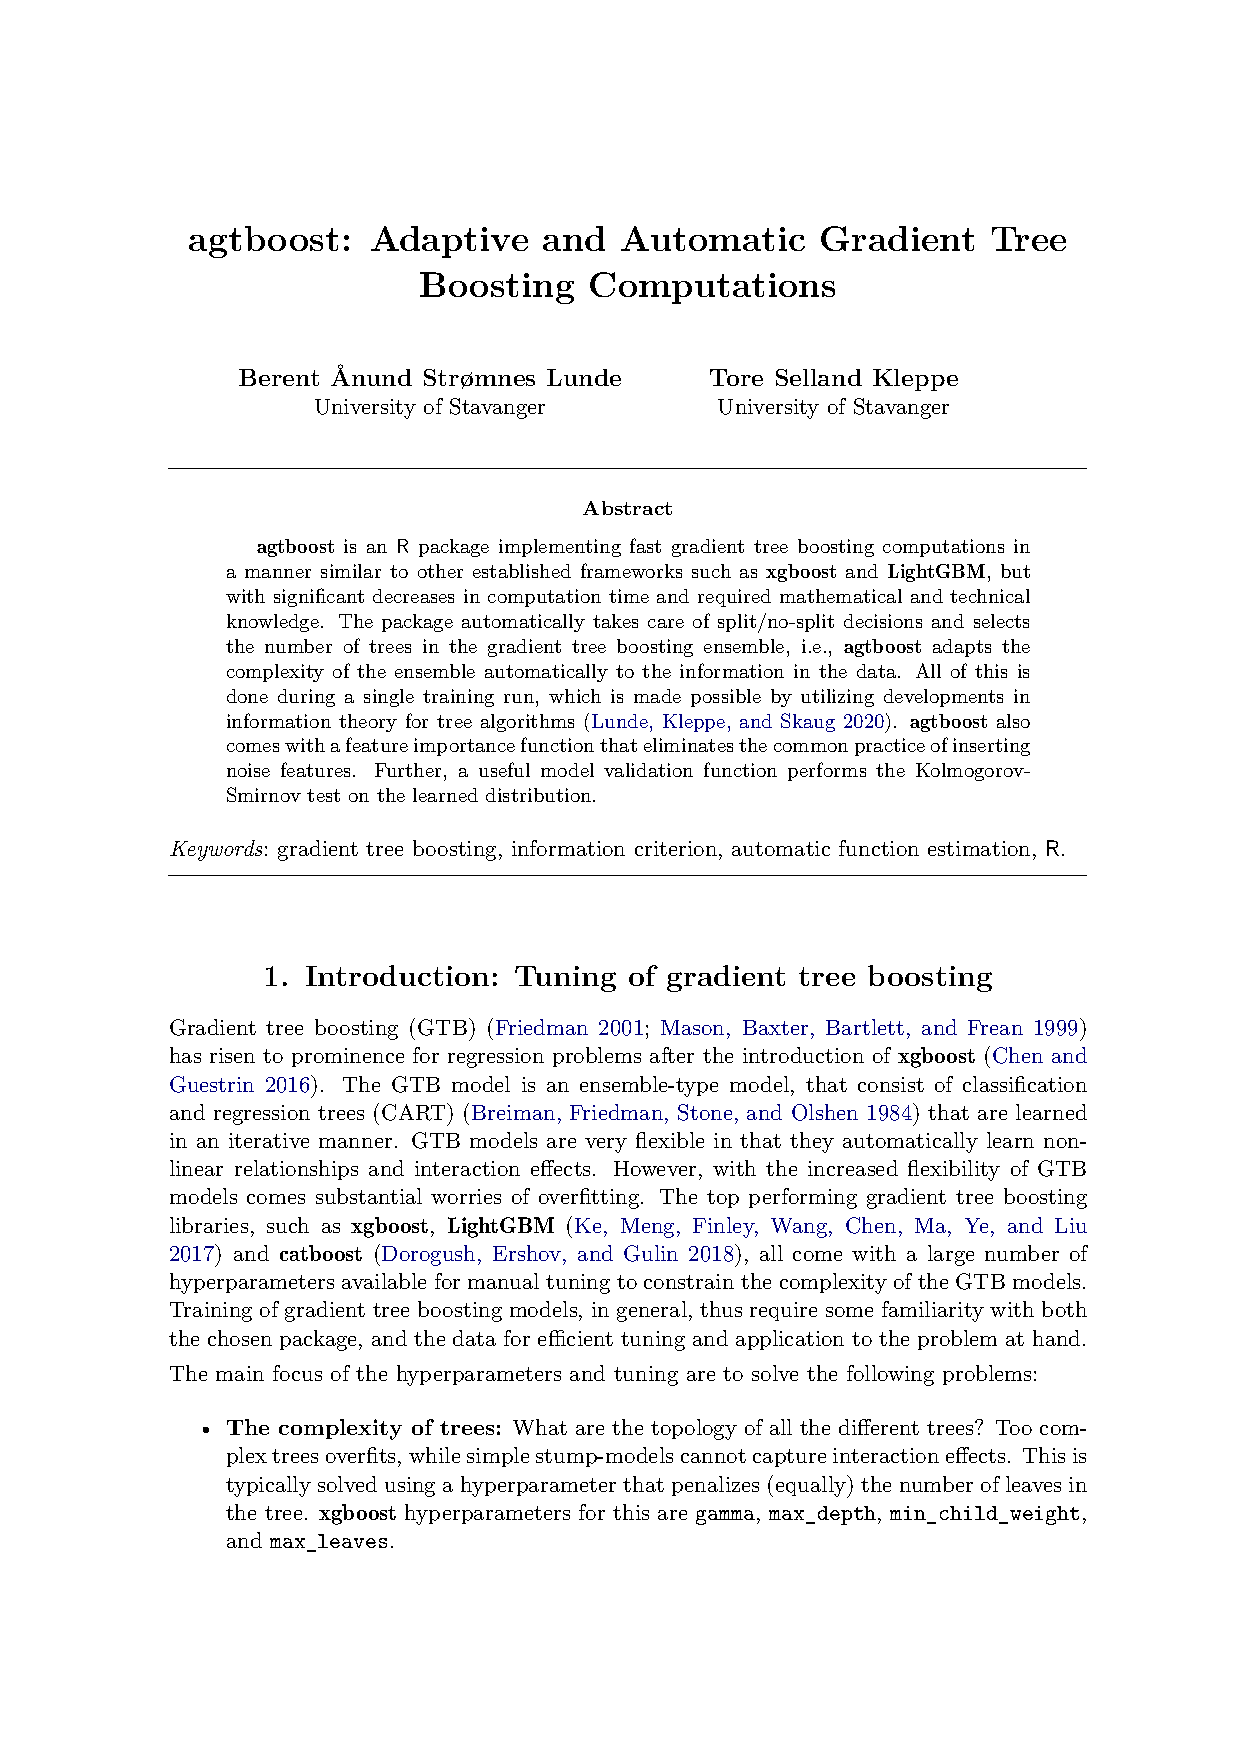
\includepdf[pages=-,scale=0.74,offset=0mm 0mm,pagecommand={\thispagestyle{plain}}]{papers/Paper3.pdf}

%%%%%%%%%%%%%%%%%%%%%%%%%%%%%%% PAPER IV %%%%%%%%%%%%%%%%%%%%%%%%%%%%%%%%%

%\insertPaper{IV}{\PaperTitleFour}
%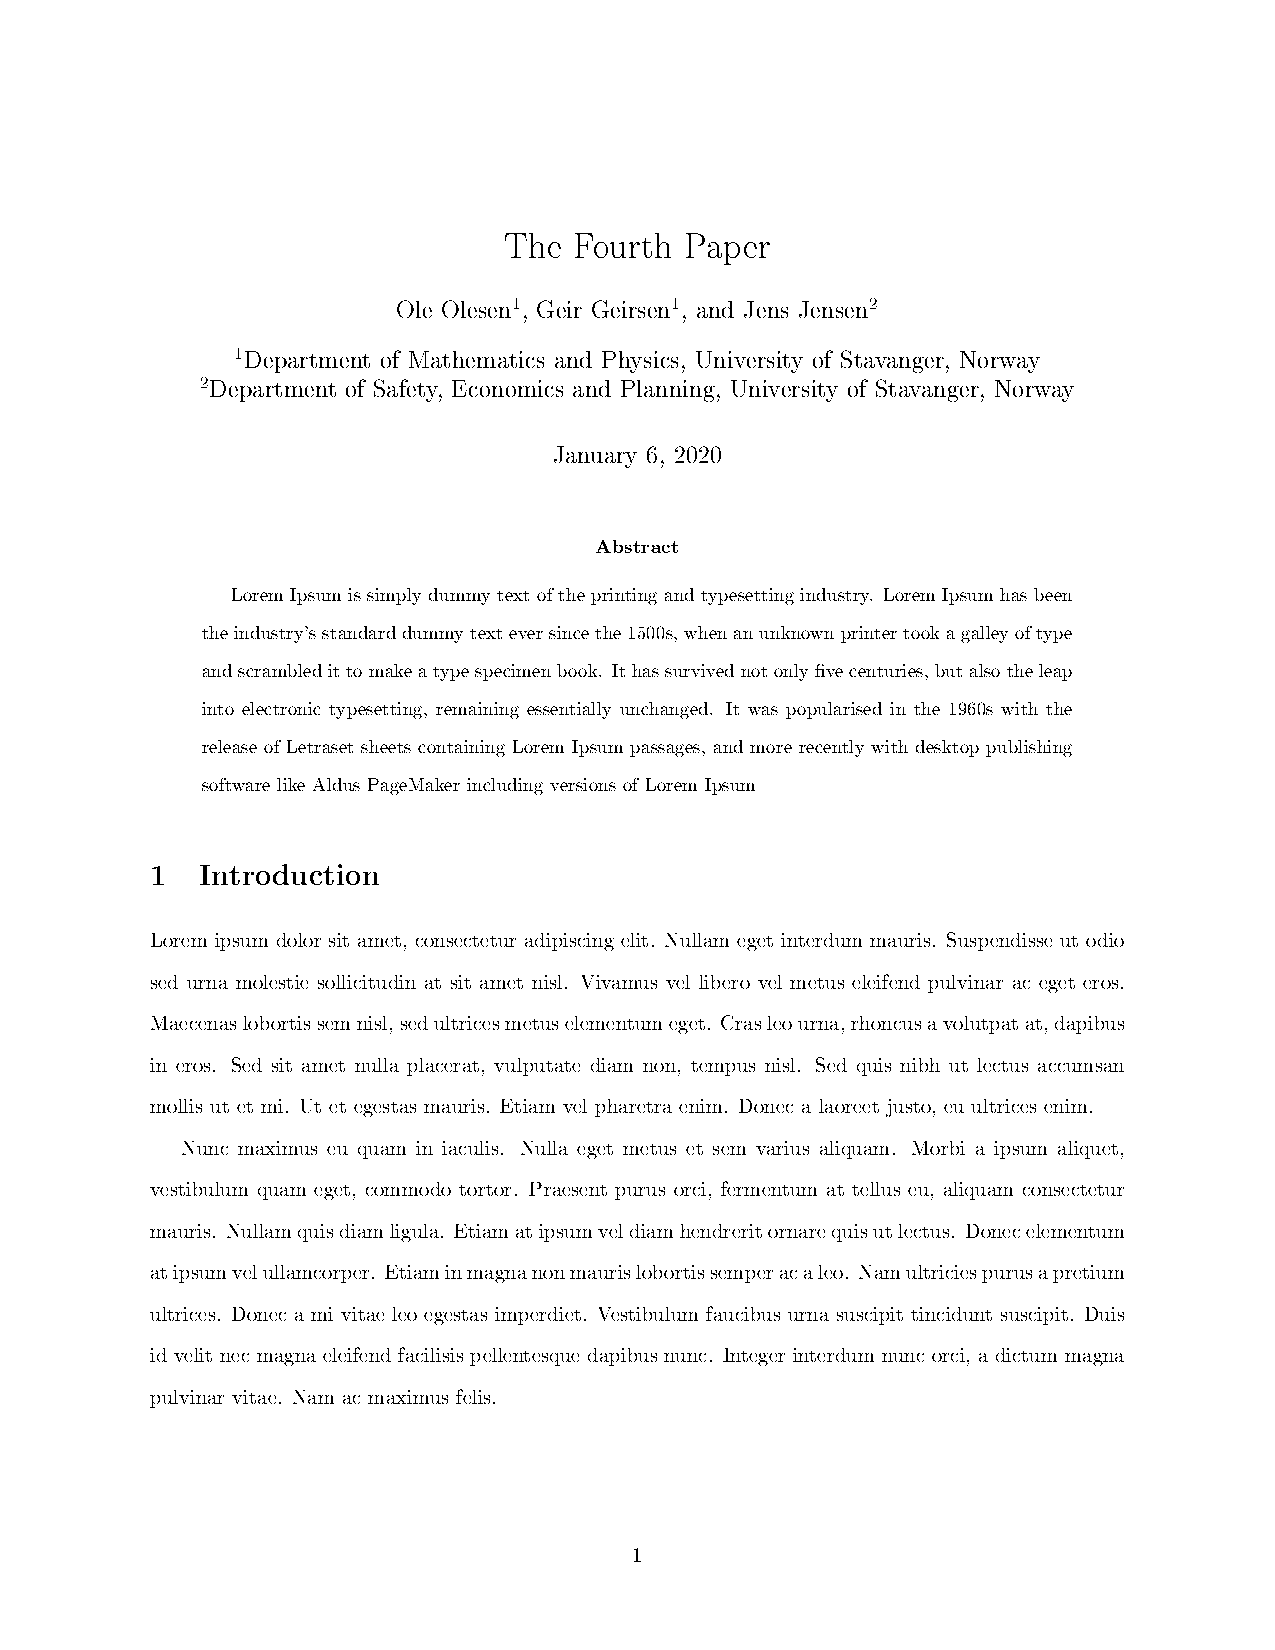
\includepdf[pages=-,scale=0.74,offset=0mm 10mm,pagecommand={\thispagestyle{plain}}]{papers/Paper4.pdf}

%%%%%%%%%%%%%%%%%%%%%%%%%%%%%%%%%%%%%%%%%%%%%%%%%%%%%%%%%%%%%%%%%%%%%%%%%%

\end{document}

